\documentclass[serif]{beamer}\usepackage[]{graphicx}\usepackage[]{color}
%% maxwidth is the original width if it is less than linewidth
%% otherwise use linewidth (to make sure the graphics do not exceed the margin)
\makeatletter
\def\maxwidth{ %
  \ifdim\Gin@nat@width>\linewidth
    \linewidth
  \else
    \Gin@nat@width
  \fi
}
\makeatother

\definecolor{fgcolor}{rgb}{0.345, 0.345, 0.345}
\newcommand{\hlnum}[1]{\textcolor[rgb]{0.686,0.059,0.569}{#1}}%
\newcommand{\hlstr}[1]{\textcolor[rgb]{0.192,0.494,0.8}{#1}}%
\newcommand{\hlcom}[1]{\textcolor[rgb]{0.678,0.584,0.686}{\textit{#1}}}%
\newcommand{\hlopt}[1]{\textcolor[rgb]{0,0,0}{#1}}%
\newcommand{\hlstd}[1]{\textcolor[rgb]{0.345,0.345,0.345}{#1}}%
\newcommand{\hlkwa}[1]{\textcolor[rgb]{0.161,0.373,0.58}{\textbf{#1}}}%
\newcommand{\hlkwb}[1]{\textcolor[rgb]{0.69,0.353,0.396}{#1}}%
\newcommand{\hlkwc}[1]{\textcolor[rgb]{0.333,0.667,0.333}{#1}}%
\newcommand{\hlkwd}[1]{\textcolor[rgb]{0.737,0.353,0.396}{\textbf{#1}}}%

\usepackage{framed}
\makeatletter
\newenvironment{kframe}{%
 \def\at@end@of@kframe{}%
 \ifinner\ifhmode%
  \def\at@end@of@kframe{\end{minipage}}%
  \begin{minipage}{\columnwidth}%
 \fi\fi%
 \def\FrameCommand##1{\hskip\@totalleftmargin \hskip-\fboxsep
 \colorbox{shadecolor}{##1}\hskip-\fboxsep
     % There is no \\@totalrightmargin, so:
     \hskip-\linewidth \hskip-\@totalleftmargin \hskip\columnwidth}%
 \MakeFramed {\advance\hsize-\width
   \@totalleftmargin\z@ \linewidth\hsize
   \@setminipage}}%
 {\par\unskip\endMakeFramed%
 \at@end@of@kframe}
\makeatother

\definecolor{shadecolor}{rgb}{.97, .97, .97}
\definecolor{messagecolor}{rgb}{0, 0, 0}
\definecolor{warningcolor}{rgb}{1, 0, 1}
\definecolor{errorcolor}{rgb}{1, 0, 0}
\newenvironment{knitrout}{}{} % an empty environment to be redefined in TeX

\usepackage{alltt}
\usetheme{Boadilla}
\usepackage{graphicx}
\usepackage[final]{animate}
\usepackage{breqn}
\usepackage{xcolor}
\usepackage{booktabs}
\usepackage{tikz}
\usetikzlibrary{decorations.pathreplacing}
\usetikzlibrary{shapes,arrows,positioning,shadows}
\usepackage{subfig}
\usepackage{pgf}

% change format of enumerated lists
\setbeamertemplate{enumerate items}[default]

\setbeamertemplate{navigation symbols}{}

% custom colors
\definecolor{mypal1}{HTML}{F0F9E8}\definecolor{mypal2}{HTML}{BAE4BC}\definecolor{mypal3}{HTML}{7BCCC4}\definecolor{mypal4}{HTML}{43A2CA}\definecolor{mypal5}{HTML}{0868AC}

\tikzstyle{decision} = [diamond, draw, text width=6em, text badly centered, inner sep = 2pt, top color=white, bottom color=mypal3, drop shadow]
\tikzstyle{block} = [rectangle, draw, text width=10em, text centered, rounded corners, minimum height=3em, minimum width=8em, top color = white, bottom color=mypal4,  drop shadow]
\tikzstyle{declare} = [rectangle, draw, text width=10em, text centered, minimum height=3em, minimum width=8em, top color = white, bottom color=mypal5,  drop shadow]

% knitr setup


% dependent data


% get online bib file


% figure used on title page


\setbeamercolor{title}{fg=mypal5} % main title
\setbeamercolor{frametitle}{fg=mypal4, bg=mypal2} % frame titles
\setbeamercolor{structure}{fg=mypal4} % bottom banner
\setbeamercolor{normal text}{fg=mypal5}
\usebackgroundtemplate{\includegraphics[height=\paperheight,width=\paperwidth]{fig/back_tmp.pdf}}

% macros
\newcommand{\emtxt}[1]{\textbf{\textit{#1}}}
\IfFileExists{upquote.sty}{\usepackage{upquote}}{}
\begin{document}

\title[Evaluating water quality]{\textbf{Quantitative approaches to understand nutrient pollution in estuaries: An example for the upper San Francisco Estuary}}
\author[M. Beck]{Marcus W. Beck, PhD}

\institute[USEPA]{USEPA National Health and Environmental Effects Research Laboratory, Gulf Ecology Division, \href{mailto:beck.marcus@epa.gov}{beck.marcus@epa.gov}, Phone: 8509342480}

\date{Aug. 26, 2016}

% \titlegraphic{\includegraphics[width=0.95\linewidth]{fig/title_plo.pdf}}

%%%%%%
\begin{frame}[shrink]
\titlepage
\end{frame}

\section{Background}

%%%%%%
\begin{frame}{\textbf{Evaluating estuarine condition}}{\textbf{How do we collect and use data?}}
\onslide<+->
The foundation of environmental management is a strong monitoring network \scriptsize \cite{NRC90}\\~\\
\normalsize
Monitoring provides information for decision-making based on apparent trends...
\vspace{0.2in}
\begin{center}
\emtxt{What are the changes in environmental condition over time?}\\~\\
\emtxt{Are these changes `good' or `bad' based on our management objectives?}\\~\\
\emtxt{What may have caused these changes?}
\end{center}
\end{frame}

%%%%%%
\begin{frame}{\textbf{Evaluating estuarine condition}}{\textbf{How do we collect and use data?}}
\onslide<+->
\emtxt{The good news}: We are getting better at monitoring - standardized, automated, increased coverage, real-time/continuous \\~\\
\emtxt{The bad news}: Our ability to use these data for decision-making has not kept pace with availability! \\~\\
\onslide<+->


{\centering \includegraphics[width=0.55\textwidth]{fig/theo-1} 

}



\end{frame}

%%%%%%
\begin{frame}{\textbf{Evaluating estuarine condition}}{\textbf{How do we collect and use data?}}
Most of my research career has focused on using monitoring data to understand effects of eutrophication in one form or another \\~\\
\onslide<+->
\begin{quote}
Eutrophication (noun) - an \emtxt{increase} in the rate of supply of \emtxt{organic matter} to an ecosystem\\
\hfill -- \cite{Nixon95}
\end{quote}
\begin{center}
\scalebox{1}{
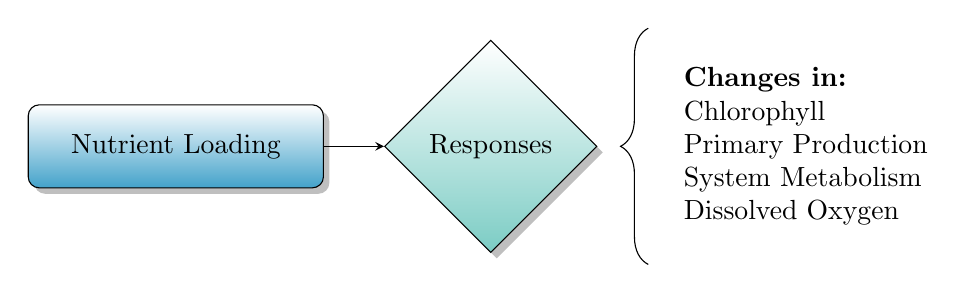
\begin{tikzpicture}[node distance = 4cm, auto, >=stealth]
  \onslide<+->{
  \node[block] (a) {Nutrient Loading};}
  \onslide<+->{
	\node[decision] (b)  [right of=a] {Responses};
 	\draw[->] (a) -- (b);}
  \onslide<+->{
  \draw[decorate,decoration={brace,amplitude=10pt}] [right of=b] (2,-1.5) -- (2,1.5);
  \node[draw,align=left,draw=none] [right of=b] {\textbf{Changes in:}\\ Chlorophyll\\ Primary Production\\ System Metabolism\\ Dissolved Oxygen};}
\end{tikzpicture}}
\end{center}
\vspace{-0.5cm}\hspace*{15pt}\scalebox{0.7}{\hbox{\tiny Adapted from \cite{Cloern01}}}\\~\\
\end{frame}

%%%%%%
\begin{frame}{\textbf{Evaluating estuarine condition}}{\textbf{How do we collect and use data?}}
\onslide<+->
\emtxt{Today's talk}: My experience evaluating monitoring data to inform our understanding of the eutrophication paradigm\\~\\
Water quality trends in the Delta: \\~\\
\begin{itemize}
\item \emtxt{Example 1}: Model theory and application \\~\\
\item \emtxt{Example 2}: Trends over time \\~\\
\item \emtxt{Example 3}: Selected case studies 
\end{itemize}
\end{frame}

\section{Model theory and background}



%%%%%%
\begin{frame}{\textbf{Model theory and background}}{\textbf{WRTDS adaptation for tidal waters}}
Increasing availability of records describing \emtxt{long-term changes} \\~\\
Observed data can provide a means to an end, potentially \emtxt{high power} with large sample size \\~\\
Can we \emtxt{develop} and \emtxt{apply} tools that leverage the descriptive capabilities of these large datasets? \\~\\
Can we \emtxt{link descriptions} to \emtxt{causal events} to inform management or understanding? \\~\\
\begin{figure}
\centerline{\includegraphics[width = \textwidth]{fig/ts_ex.pdf}}
\end{figure}
\end{frame}

%%%%%%
\begin{frame}[t]{\textbf{Model theory and background}}{\textbf{WRTDS adaptation for tidal waters}}
{\bf \centerline{Observed data represents effects of many processes}}
\vspace{0.2in}
\centerline{\includegraphics[width = \textwidth]{fig/ts_ex.pdf}}
\vspace{0.2in}
\begin{columns}[t]
\begin{column}{0.3\textwidth}
{\bf \underline{\emtxt{Climate}}}\\
precipitation\\
temperature\\
wind events\\
ENSO effects
\end{column}
\begin{column}{0.3\textwidth}
{\bf \underline{\emtxt{Local}}}\\
light/turbidity\\
residence time\\
invasive species\\
trophic effects
\end{column}
\begin{column}{0.3\textwidth}
{\bf \underline{\emtxt{Regional/historical}}}\\
watershed inputs\\
point sources\\
management actions
flow changes
\end{column}
\end{columns}
\end{frame}

%%%%%%
\begin{frame}[t]{\textbf{Model theory and background}}{\textbf{WRTDS adaptation for tidal waters}}
\onslide<+->
{\bf \centerline{Observed data represents effects of many processes}}
\vspace{0.2in}
\centerline{\includegraphics[width = \textwidth]{fig/ts_ex.pdf}}
\centerline{Models should describe components to evaluate effects}
\vspace{-0.1in}
\begin{columns}[t]
\begin{column}{0.5\textwidth}
\onslide<+->{
\centerline{\includegraphics[width = 0.8\textwidth]{fig/schematic2.pdf}}
\centerline{\includegraphics[width = 0.8\textwidth]{fig/schematic3.pdf}}
}
\end{column}
\begin{column}{0.5\textwidth}
\onslide<+->{
\centerline{\includegraphics[width = 0.8\textwidth]{fig/schematic4.pdf}}
\centerline{\includegraphics[width = 0.8\textwidth]{fig/schematic5.pdf}}
}
\end{column}
\end{columns}
\end{frame}

%%%%%%
\begin{frame}[t]{\textbf{Model theory and background}}{\textbf{WRTDS adaptation for tidal waters}}
\emtxt{Problem:} Response endpoints of eutrophication vary naturally over time and with discharge or tidal patterns\\~\\
\emtxt{Solution:} Develop a model that accounts for changes in relationships between drivers of pollution over time\\~\\
The \emtxt{weighted regression (WRTDS)} model is being developed by USGS for pollutant modelling in rivers \cite{Hirsch10}\\~\\
Models pollution concentration as a function of \emtxt{time}, \emtxt{discharge}, and \emtxt{season}\\~\\
\emtxt{Adaptation:} Applied to Tampa Bay \cite{Beck15}, further validated/compared in Patuxent Estuary [Beck and Murphy, In review]
\end{frame}



%%%%%%
\begin{frame}{\textbf{Model theory and background}}{\textbf{WRTDS adaptation for tidal waters}}
How does weighted regression work?
\begin{center}
\animategraphics[controls,width=\linewidth]{10}{fig/wtex}{}{} %frame rate is 12 per/sec
\end{center}
\end{frame}
 

 
%%%%%%
\begin{frame}{\textbf{Model theory and background}}{\textbf{WRTDS adaptation for tidal waters}} 
Application to Delta:\\~\\
\begin{columns}
\begin{column}{0.4\textwidth}
\begin{itemize}
\item Nine stations (three Suisun, three middle, three delta) \\~\\
\item Three analytes (DIN, ammonium, nitrite/nitrate), two flow records \\~\\
\item Four decades of data
\end{itemize}
\end{column}
\begin{column}{0.5\textwidth}
\centerline{\includegraphics[width = \textwidth]{fig/stations.pdf}}
\end{column}
\end{columns}
\end{frame}

%%%%%%
\begin{frame}
Acknowledgments:\\~\\
\begin{columns}
\begin{column}{0.8\textwidth}
{\footnotesize
Research staff and employees at USEPA Gulf Ecology Division \\~\\
}
\end{column}
\begin{column}{0.2\textwidth}
\end{column}
\end{columns}
\vfill
Funding sources and contact:\\~\\
\begin{columns}
\begin{column}{0.5\textwidth}
\centerline{\includegraphics[width=0.4\linewidth]{fig/epa_logo.png}}
\end{column}
\begin{column}{0.5\textwidth}
\scriptsize
\href{mailto:beck.marcus@epa.gov}{beck.marcus@epa.gov} \\~\\
Phone: 8509342480
\end{column}
\end{columns}
\vspace{0.2in}
\end{frame}

%%%%%%
\section{References}
\begin{frame}[t]{\textbf{References}}
\tiny
\setbeamertemplate{bibliography item}{}
\bibliographystyle{apalike_mine}
\bibliography{refs}
\end{frame}

\end{document}
